\subsubsection*{Informazioni sul package}
	Il package serve per far comunicare le view con il model in entrambe le direzioni ovvero rendere visibili gli aggiornamenti del model nella view e viceversa aggiornare il model con le informazioni provenienti dalla view.
		\begin{figure}[h]
			\centering
			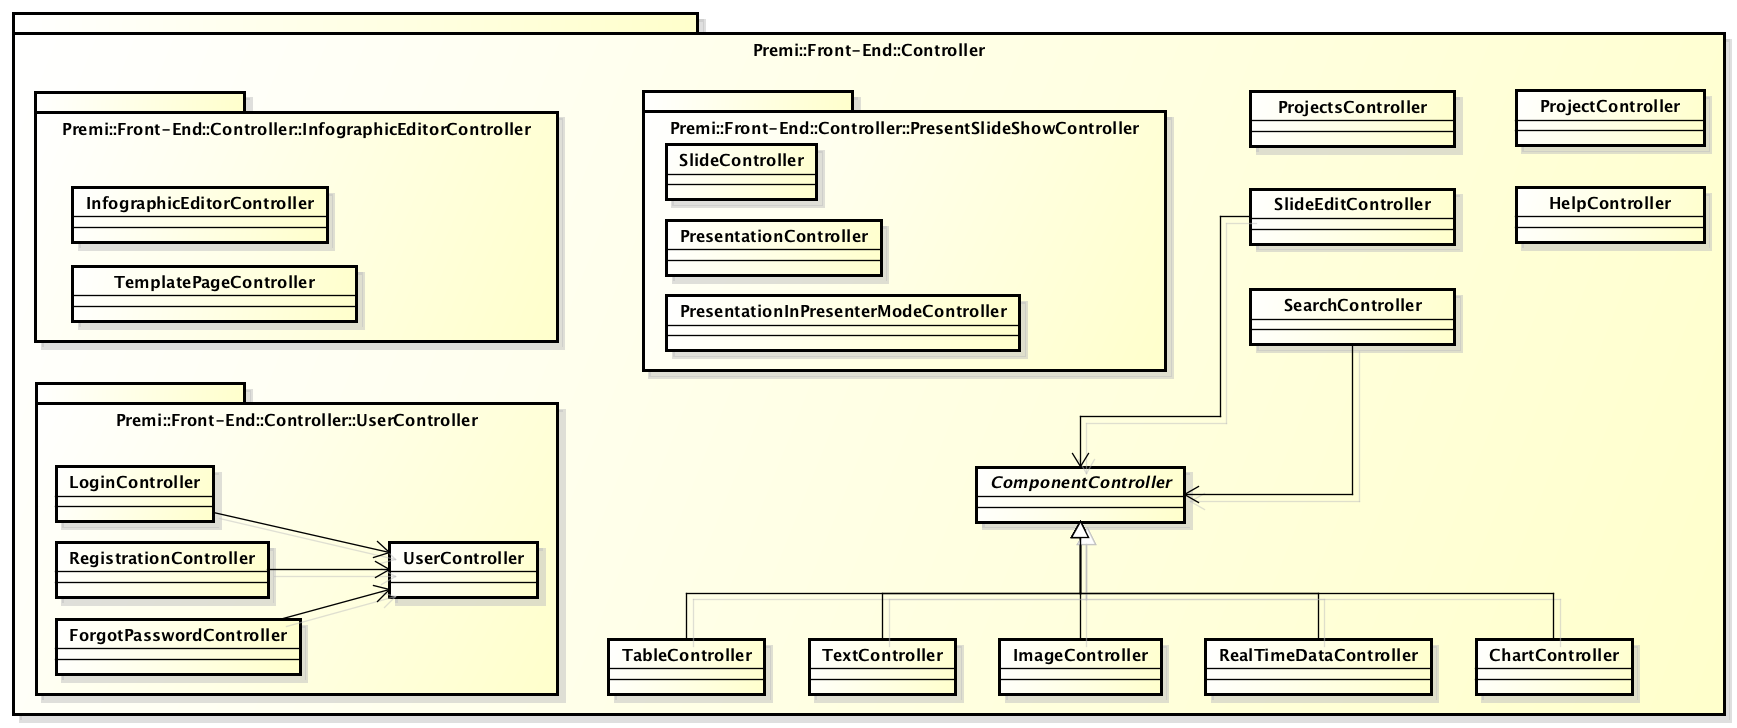
\includegraphics[width=1.0\linewidth]{img/front-end_controller}
			\caption[Premi::Front-End::Controller]{Premi::Front-End::Controller}
		\end{figure}
	\subsubsection*{Package contenuti}
		\begin{itemize}
		 \item Premi::Front-End::Controller::PresentSlideShowController
		 \begin{itemize}
		    \item Package per la gestione dell'editor per le presentazioni.
		 \end{itemize}
		 \item Premi::Front-End::Controller::InfographicEditorController
		 \begin{itemize}
		    \item Package per la gestione dell'editor per le infografiche.
		 \end{itemize}
		 \item Premi::Front-End::Controller::UserController
		 \begin{itemize}
		    \item Package per la gestione degli utenti.
		 \end{itemize}
		\end{itemize}
	\subsubsection*{Classi contenute}
		\begin{itemize}
		 \item Premi::Front-End::Controller::ProjectsController:
			\begin{itemize}
				\item \textbf{Descrizione}: classe con lo scopo di fornire le operazioni necessarie alla visualizzazione e gestione dei progetti relativi ad un utente.
			\end{itemize}
		\item  Premi::Front-End::Controller::ProjectController: 
			 \begin{itemize}
				\item \textbf{Descrizione}: classe con lo scopo di fornire le operazioni necessarie alla visualizzazione e gestione di un progetto.
			\end{itemize}
		\item  Premi::Front-End::Controller::SlideEditController: 
			 \begin{itemize}
				\item \textbf{Descrizione}: classe con lo scopo di fornire le operazioni necessarie alla visualizzazione e gestione dell'editor per che permette di assemblare e modificare una \gls{slide}. Il metodi che effettueranno le operazioni sui componenti, utilizzeranno il pattern command per la selezione della tipologia del componente.
				\item \textbf{Relazioni con altre classi}:
				\begin{itemize}
					\item Premi::Front-End::Controller::ComponentController.
				\end{itemize}
			\end{itemize}
		\item  Premi::Front-End::Controller::SearchController: 
			 \begin{itemize}
				\item \textbf{Descrizione}: classe con lo scopo di fornire le operazioni necessarie alla ricerca di progetti e presentazioni.
			\end{itemize}
		\item  Premi::Front-End::Controller::HelpController: 
			 \begin{itemize}
				\item \textbf{Descrizione}: classe con lo scopo di fornire le operazioni necessarie alla visualizzazione e gestione dell'aiuto agli utenti.
			\end{itemize}
		\item  Premi::Front-End::Controller::ComponentController: 
			 \begin{itemize}
				\item \textbf{Descrizione}: classe astratta con lo scopo di fornire le operazioni necessarie alla visualizzazione di un componente di una \gls{slide}.
			\end{itemize}
		\item  Premi::Front-End::Controller::TextController: 
			 \begin{itemize}
				\item \textbf{Descrizione}: classe con lo scopo di fornire le operazioni necessarie alla visualizzazione e gestione di un componente testuale.
				\item \textbf{Relazioni con altre classi}:
				\begin{itemize}
					\item Premi::Front-End::Controller::ComponentController.
				\end{itemize}
			\end{itemize}
		\item  Premi::Front-End::Controller::ImageController: 
			 \begin{itemize}
				\item \textbf{Descrizione}: classe con lo scopo di fornire le operazioni necessarie alla visualizzazione e gestione di una immagine.
				\item \textbf{Relazioni con altre classi}:
				\begin{itemize}
					\item Premi::Front-End::Controller::ComponentController.
				\end{itemize}
			\end{itemize}
		\item  Premi::Front-End::Controller::ChartController: 
			 \begin{itemize}
				\item \textbf{Descrizione}: classe con lo scopo di fornire le operazioni necessarie alla visualizzazione e gestione di grafici.
				\begin{itemize}
					\item Premi::Front-End::Controller::ComponentController.
				\end{itemize}
			 \end{itemize}
		\item  Premi::Front-End::Controller::TableController: 
			 \begin{itemize}
				\item \textbf{Descrizione}: classe con lo scopo di fornire le operazioni necessarie alla visualizzazione e gestione di tabelle, esse possono contere altre tabelle.
				\item \textbf{Relazioni con altre classi}:
				\begin{itemize}
					\item Premi::Front-End::Controller::ComponentController.
				\end{itemize}
			\end{itemize}
		\item  Premi::Front-End::Controller::RealTimeDataController: 
			 \begin{itemize}
				\item \textbf{Descrizione}: classe con lo scopo di fornire le operazioni necessarie alla visualizzazione e gestione di componenti aggiornate in tempo reale.
				\item \textbf{Relazioni con altre classi}:
				\begin{itemize}
					\item Premi::Front-End::Controller::ComponentController.
				\end{itemize}
			\end{itemize}
			
		\end{itemize}
		
\newpage
\subsection{Premi::Front-End::Controller::PresentSlideShowController}
\begin{figure}[h]
\centering
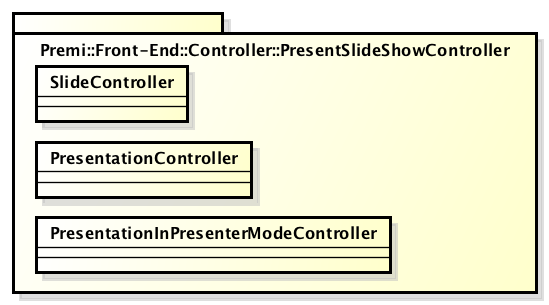
\includegraphics[width=0.7\linewidth]{img/front-end_controller_presentslideshowcontroller}
\caption[Premi::Front-End::Controller::PresentSlideShowController]{Premi::Front-End::Controller::PresentSlideShowController}
\label{fig:front-end_controller_presentslideshowcontroller}
\end{figure}

	\begin{itemize}
		 \item Premi::Front-End::Controller::PresentSlideShowController::SlideController:
			\begin{itemize}
				\item \textbf{Descrizione}: classe con lo scopo di fornire le operazioni necessarie alla visualizzazione e gestione di una \gls{slide}.
			\end{itemize}
		\item  Premi::Front-End::Controller::PresentSlideShowController::PresentationController: 
			 \begin{itemize}
				\item \textbf{Descrizione}: classe con lo scopo di fornire le operazioni necessarie alla visualizzazione e gestione di una presentazione.
			\end{itemize}
		\item Premi::Front-End::Controller::PresentSlideShowController::PresentationInPresenterModeController:
			\begin{itemize}
				\item \textbf{Descrizione}: classe con lo scopo di fornire le operazioni necessarie alla visualizzazione e gestione di una presentazione nella modalità presentatore. 
				\\Questa modalità permette al presentatore di avere degli aiuti per il suo intervento.
			\end{itemize}
	\end{itemize}
	
\newpage	
\subsection{Premi::Front-End::Controller::InfographicEditorController}
\begin{figure}[h]
\centering
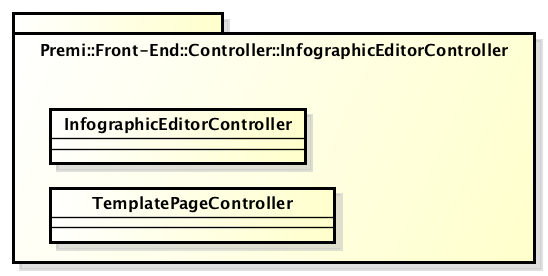
\includegraphics[width=0.7\linewidth]{img/front-end_controller_infographiceditorcontroller}
\caption[Premi::Front-End::Controller::InfographicEditorController]{Premi::Front-End::Controller::InfographicEditorController}
\label{fig:front-end_controller_infographiceditorcontroller}
\end{figure}

	\begin{itemize}
		 \item Premi::Front-End::Controller::InfographicEditorController::InfographicEditorController:
			\begin{itemize}
				\item \textbf{Descrizione}: classe con lo scopo di fornire le operazioni necessarie alla visualizzazione e gestione dell'editor per la realizzazione di una \gls{infografica}, gestendo in particolare ordine e selezione delle \gls{slide} da rappresentare.
			\end{itemize}
		\item  Premi::Front-End::Controller::InfographicEditorController::TemplatePageController: 
			 \begin{itemize}
				\item \textbf{Descrizione}: classe con lo scopo di fornire le operazioni necessarie alla visualizzazione e gestione di un \gls{template} in grado di accogliere \gls{slide} per comporre una \gls{infografica}.
			\end{itemize}
	\end{itemize}
	
\subsection{Premi::Front-End::Controller::UserController}
\begin{figure}[h]
\centering
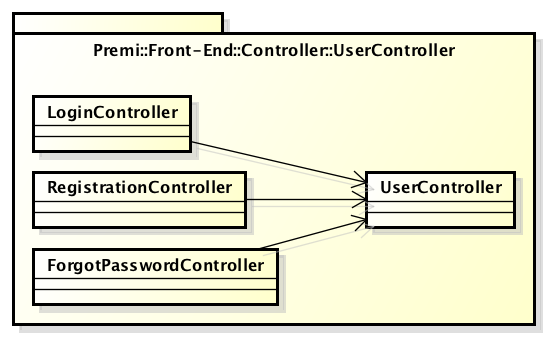
\includegraphics[width=0.7\linewidth]{img/front-end_controller_usercontroller}
\caption[Premi::Front-End::Controller::UserController]{Premi::Front-End::Controller::UserController}
\label{fig:front-end_controller_usercontroller}
\end{figure}

	\begin{itemize}
		% \item Premi::Front-End::Controller::UserController::UserController:
		%	\begin{itemize}
		%		\item \textbf{Descrizione}: classe con lo scopo di fornire le operazioni necessarie alla gestione di un utente.
		%	\end{itemize}
		\item  Premi::Front-End::Controller::UserController::LoginController: 
			 \begin{itemize}
				\item \textbf{Descrizione}: classe con lo scopo di fornire le operazioni necessarie alla visualizzazione e gestione della pagina di login.
			\end{itemize}
		 \item Premi::Front-End::Controller::UserController::RegistrationController:
			\begin{itemize}
				\item \textbf{Descrizione}: classe con lo scopo di fornire le operazioni necessarie alla visualizzazione e gestione della pagina di registrazione.
			\end{itemize}
		\item  Premi::Front-End::Controller::UserController::ForgotPasswordController: 
			 \begin{itemize}
				\item \textbf{Descrizione}: classe con lo scopo di fornire le operazioni necessarie alla visualizzazione e gestione della pagina di recupero password.
			\end{itemize}
	\end{itemize}
